\documentclass[a4paper,12pt]{article}
\usepackage[utf8]{inputenc}
\usepackage{polski}
\usepackage[left=2.5cm,right=2.5cm,top=2.5cm,bottom=2cm]{geometry}
\usepackage{mathtools}
\usepackage{amsmath}
\usepackage{latexsym}
\usepackage{url}
\usepackage{hyperref}

\title{Sprawozdanie P1.4}
\author{Kamil Tasarz, 322492}
\date{październik-listopad 2021}

\begin{document}

\maketitle


\section{Wstęp}

Stała Eulera, zwana również stałą Eulera-Mascheroniego jest stałą matematyczną oznaczaną $\gamma =  0.577215664901532286 \dots$ Jest zdefiniowana za pomocą granicy 
$$\gamma := \lim_{n-> \infty} \gamma_n,$$ $$\text{gdzie }\gamma_n := 1 + \frac{1}{2} + \frac{1}{3} + \dots + \frac{1}{n} - \ln{n}.$$
Zakładając prawdziwość przybliżenia $$\gamma_n - \gamma \approx cn^{-d}$$ dla dostatecznie dużych n, doświadczenie ma na celu wyznaczyć stałe $c, d >0$. W tym sprawozdaniu omówię etapy i wyniki tego doświadczenia.


\section{Nieco o regresji liniowej}

Regresja liniowa jest metodą szacowania jednej zmiennej, gdy dysponujemy wartościami innej zmiennej przy założeniu, ze zmienne te są od siebie zależne liniowo. Weźmy równanie liniowe
$$ y = \beta_0 + \beta_1x. $$
Chcemy dla pewnego zbioru danych, które mamy znaleźć współczynniki $\beta_0$, $\beta_1$. Dane są postaci $(x_i, y_i)$. Zapiszmy to w postaci układu:

$\begin{cases}
y_1 = \beta_0 +\beta_1x_1 + \epsilon_1 \\
y_2 = \beta_0 +\beta_1x_2 + \epsilon_2 \\ 
\hspace{6mm} \vdots \\
y_n = \beta_0 +\beta_1x_n + \epsilon_n,
\end{cases}$

\noindent gdzie $\epsilon_i$ to błąd, który należy zminimalizować dobierając odpowiednie $\beta_0$, $\beta_1$. \\
Niech:
$$
Y = \begin{pmatrix} y_1 \\ y_2 \\ \vdots \\ y_n \end{pmatrix}, \quad
X = \begin{pmatrix} 1 & x_1 \\ 1 & x_2 \\ \vdots & \vdots \\ 1 & x_n \end{pmatrix}, \quad
B = \begin{pmatrix} \beta_0 \\ \beta_1 \end{pmatrix} \quad
\text{oraz} \quad
E = \begin{pmatrix} \epsilon_1 \\  \epsilon_2 \\ \vdots \\  \epsilon_n \end{pmatrix}
$$
Możemy teraz zapisac nasz układ w postaci macierzowej
$$ Y = XB + E .$$
Chcielibyśmy zminimalizować $\sum_{i=1}^n\epsilon_i$.
Mamy $$ \sum_{i=1}^n\epsilon_i^2 = \sum_{i=1}^n(\beta_0 + \beta_1x_i - y_i)^2 $$
czyli $$ 0 = \sum_{i=1}^n(\beta_0 + \beta_1x_i - y_i)^2 - \sum_{i=1}^n\epsilon_i^2. $$
Funckja ta osiąga swoje minimum w miejscu zerowania się pochodnych. Znajdźmy te punkty. Najpierw zróżniczkujmy po $\beta_0 $ i $\beta_1$.
$$ 0 = \sum_{i=1}^n 2  (\beta_0 + \beta_1x_i - y_i) $$
$$ 0 = \sum_{i=1}^n 2  x_i (\beta_0 + \beta_1x_i - y_i) $$
Po rozdzieleniu sum i uporządkowaniu dostajemy układ:
$$ \beta_0 \sum_{i=1}^n 1 + \beta_1 \sum_{i=1}^n x_i = \sum_{i=1}^n y_i $$
$$ \beta_0 \sum_{i=1}^n x_1 + \beta_1 \sum_{i=1}^n x_i^2 = \sum_{i=1}^n x_iy_i $$
A po zapisaniu w postaci macierzowej:
$$
\begin{pmatrix} \sum 1 & \sum x_i \\
\sum x_i & \sum x_i^2 \end{pmatrix} 
\begin{pmatrix} \beta_0 \\ \beta_1 \end{pmatrix}
=
\begin{pmatrix} \sum y_i \\ \sum x_iy_i \end{pmatrix} 
$$
Zauważmy, że dla wcześniej zdefiniowanych macierzy
$$
Y = \begin{pmatrix} y_1 \\ y_2 \\ \vdots \\ y_n \end{pmatrix}, \quad
X = \begin{pmatrix} 1 & x_1 \\ 1 & x_2 \\ \vdots & \vdots \\ 1 & x_n \end{pmatrix}
$$
zachodzą równości
$$
\begin{pmatrix} \sum 1 & \sum x_i \\
\sum x_i & \sum x_i^2 \end{pmatrix}  =
\begin{pmatrix} 1 & 1 & \cdots & 1 \\
x_1 & x_2 & \cdots & x_n \end{pmatrix}
\begin{pmatrix} 1 & x_1 \\ 1 & x_2 \\ \vdots & \vdots \\ 1 & x_n \end{pmatrix}
=
XX^{T}
$$
oraz
$$
\begin{pmatrix} \sum y_i \\ \sum x_iy_i \end{pmatrix}
=
\begin{pmatrix} 1 & 1 & \cdots & 1 \\
x_1 & x_2 & \cdots & x_n \end{pmatrix}
\begin{pmatrix} y_1 \\ y_2 \\ \vdots \\ y_n \end{pmatrix}
=
X^{T}Y
$$
Po wstawieniu do równania otrzymujemy:
$$ X^{T}XB = X^{T}Y, $$
a po przekształceniu:
\begin{equation} B = (X^{T}X)^{-1}X^{T}Y  \end{equation}
Jest to wzór na takie $\beta_0$, $\beta_1$, dla których suma $\epsilon_i$ będzie najmniejsza. Czyli są to współczynniki najlepiej oddające zależność liniową $ y = \beta_0 + \beta_1x$ dla danego zbioru zmiennych $(x_i, y_i)$.


\section{Powiązanie z zadaniem}

Uznajmy za prawdziwe przybliżenie
$$ \gamma_n - \gamma \approx cn^{-d}. $$
Po zlogarytmowaniu dostajemy 
$$ \ln(\gamma_n - \gamma) \approx -d\ln(n) + \ln(c).$$
Jeśli potraktujemy $\ln(\gamma_n - \gamma)$ jako zmienną $y$, $\ln(n)$ jako zmienną $x$, a szukane $\ln(c)$ oraz $-d$ kolejno jako współczynniki $\beta_0$ i $\beta_1$. Dostajemy równanie (właściwie przybliżenie) liniowe. Kolejno korzystając ze wzoru (1), gdzie $B = \begin{pmatrix} \ln(c) \\ -d \end{pmatrix}$, dla dostatecznie dużych n możemy wyznaczyć doświadczalnie przybliżenie stałych $c$ i $d$.


\section{Program i pierwsze wyniki}

Program jest napisany w języku Julia w wersji 1.6.3. Do obliczeń będę używał precyzji 256-bitowej, która zapewnia wystarczającą dokładność do osiągnięcia celu.
Weźmy kilka macierzy X, odpowiadajace im macierze Y i policzmy macierz B.
Niech macierz X składa się z dziesięciu elementów $x_i$ od $10^i$ do $10^{i+1}$, czyli np. dla $i=3$ będą to liczby: $1000, 2000, 3000, \dots, 10 000$.

\begin{center}
$\begin{array}{|c|l|l|l|} \hline
i & \ln(c) & e^{\ln(c)} = c & d \\ \hline
1 & -0.7209 \dots & 0.4862 \dots & -0.9939 \dots \\ \hline
2 & -0.69728 \dots & 0.49793 \dots & -0.99940 \dots \\ \hline
3 & -0.693698 \dots & 0.49972 \dots & -0.999940 \dots \\ \hline
4 & -0.693216 \dots & 0.499965 \dots & -0.9999940 \dots \\ \hline
5 & -0.693155 \dots & 0.49999587 \dots & -0.99999940 \dots \\ \hline
6 & -0.6931481 \dots & 0.499999506 \dots & -0.9999999387 \dots \\ \hline
7 & -0.69314676 \dots & 0.500000209 \dots & -1.0000000238 \dots \\ \hline
\end{array}$
\end{center}
Już te kilka wyników pozwala nam przypuszczać, że szukane to $d = 1$ oraz $c = 0.5$.

\section{Potwierdzenie oszacowania}
Udało nam się oszacować stałe $c$ oraz $d$. Załóżmy, że są one poprawne, to jest, zgodnie z treścią naszego zadania, dla dostatecznie dużych n, zachodzi
$$ \gamma_n - \gamma \approx \frac{1}{2n}. $$
Sprawdźmy jak zachowuje się wyrażenie $ \omega(n) = \gamma_n - \gamma - \frac{1}{2n}.$ \\
Jeśli stałe są wyznaczone dobrze to wyrażenie to powinno być w przybliżeniu równe $0$ dla dużych $n$. Zobaczmy wykres:

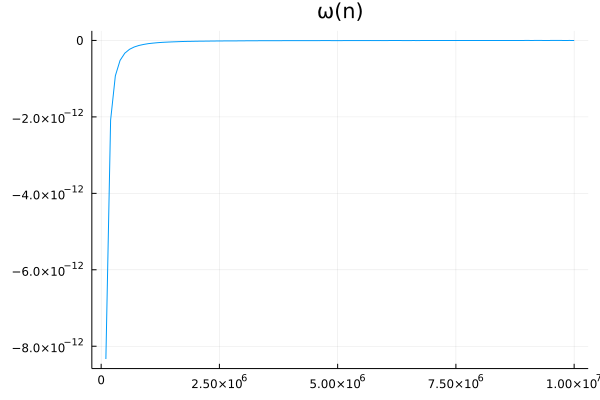
\includegraphics[width=13cm]{wyk.png}

\noindent Pomimo tego, że $\omega(1)$ jest rzędu $10^{-2}$ to zbliża się ona do zera szybko. Dla $n$ rzędu $10^4$ $\omega(n)$ jest rzędu $10^{-10}$. Wykres przedstawia wartości dla jeszcze większych $n$.


\section{Podsumowanie}

W tym doświadczeniu udało mi przybliżyć wyrażenie $\gamma_n - \gamma \approx \frac{1}{2n}$. Posłużyłem się metodą regresji liniowej wykorzystywanej w statystyce. Wyprowadziałem ogólny wzór i zastosowałem go do danego problemu. Na koniec, mając podejrzenia co do wartości szukanych stałych, sprawdziłem jak dobrze przybliżają one wyrażenie $\gamma_n - \gamma$.  


\begin{thebibliography}{9}
\bibitem{texbook}
Using matrix algebra in linear regresssion, Jackie Nicholas, Mathematics Learning Centre, University of Sydney (2010) -  \href{https://www.sydney.edu.au/content/dam/students/documents/mathematics-learning-centre/using-matrix-algebra-in-linear-regression.pdf}{link}

\bibitem{lamport94}
Bo Li's lecture script -  \href{https://www.stat.purdue.edu/~boli/stat512/lectures/topic3.pdf}{link}
\end{thebibliography}

\end{document}
